% 导言

% 文类
\documentclass[a4paper, onecolumn, 10pt, space]{ctexart}

% 宏包调用
%\usepackage[space]{ctex}
%\usepackage{xeCJK}
\usepackage{cchess}
\usepackage{texnames}
\usepackage{lipsum}
\usepackage{blindtext}
\usepackage{graphicx}
\usepackage{xcolor}
\usepackage{fancybox}
\usepackage{lineno}
\usepackage{graphpap}
\usepackage{listings}
\usepackage{comment}
\usepackage{draftwatermark}
%\usepackage{xwatermark}
\usepackage{evenpage}
\usepackage{layout}
\usepackage{lscape}
\usepackage[pagecolor=none]{pagecolor}
\usepackage{tikz}
\usepackage{ulem}
\usepackage{lettrine}
\usepackage[stable]{footmisc}

\usetikzlibrary{calc}

% 设置
\SetWatermarkText{FlushHip}
\SetWatermarkLightness{0.9}
\SetWatermarkScale{0.2}
\SetWatermarkHorCenter{450pt}
\SetWatermarkVerCenter{700pt}

\setcounter{secnumdepth}{4}

\listfiles

% 正文
\begin{document}

\setlength{\parindent}{0pt}
\setlength{\columnsep}{3em}
\setlength{\columnseprule}{0.4pt}

\begin{abstract}
    学习\LaTeXe{}
\end{abstract}

\begin{center}
    \large \METAFONT{}
\end{center}

\vspace{2em}

\noindent{}\LaTeXe{}忽略命令后的一切空格,因此如需保留空格,可在命令后加\verb"{"\verb"}"\textvisiblespace{}或者\verb"\"\textvisiblespace{}。\LaTeX\

命令中的参数
\begin{itemize}
    \item 必要参数 \textbraceleft{params}\textbraceright{}
    \item 可选参数 [params]
\end{itemize}

根据命令不同的作用范围,可以把命令分成下面四种
\begin{itemize}
    \item 声明形式:将作用于命令之后的所有相关内容,如{\bfseries 粗体命令}
    \item 参数形式:只作用与命令所带参数,如斜体命令\textsl{Asia}
    \item 组合形式:加\{\ \}限定声明形式的作用域,如{\bfseries \{Asia\}}
    \item 环境形式
\end{itemize}

\newcommand{\name}{FlushHip}
In 1971, \name{} nice!

\newcommand{\shulie}[2][n]{\(#2_1, #2_2, \dots, #2_#1\)}
\shulie{x}, \shulie[m]{a}

\ensuremath{x^2 + y^2 = z^2}

排版模式
\begin{itemize}
    \item 左右模式 \mbox{\bfseries 左右模式啦啦啦}
    \item 段落模式\ 最常用的模式,分段、分页,系统默认排版模式
    \item 数学模式~字体变斜体,忽略所有符号之间的空白\(\pi ^ 2\)
\end{itemize}

中文排版中,所有标点符号都使用全角逗号和空心句号,数学式中才使用半角逗号。

相对长度单位em用于水平长度设置,ex用于垂直长度设置。

\framebox[20em][l]{左 \hspace{\fill} 右}\\
\framebox[20em][l]{左 \hfill 中 \hfill 右}\\
\framebox[20em][l]{左 \hfil 中 \hfill 右}

\fbox{
    \parbox[c][20mm][t]{1em}{上 \vfill 中 \vfill 下}
}
\fbox{
    \parbox[c][20mm][t]{1em}{上 \vfil 中 \vfill 下}
}

\the\parindent{}

\makebox[6cm]{\dotfill}
\makebox[6cm]{\hrulefill}
\makebox[6cm]{\downbracefill}
\makebox[6cm]{\upbracefill}
\makebox[6cm]{\leftarrowfill}
\makebox[6cm]{
    \fbox{\shortstack{左边 \\ 文本}}
    \rightarrowfill{}
    \fbox{\shortstack{右边 \\ 文本}}
}

每个字符就是一个盒子,左右盒子、段落盒子、线段盒子。盒子是一个不可分割的整体,因此不能跨行和跨页。

\fbox{
    \shortstack{
        \makebox[60mm][s]{电子计算机}\\
        \makebox[60mm][s]{computer}\\
        \makebox[60mm][s]{c o m p u t e r}
    }
}

\parindent=2em
For emphasis, you may wish to \raisebox{1.5ex}{rasie} or \raisebox{-1.5ex}{lower} certain text inside you document.

\makebox[0pt][r]{\fbox{注意}} \blindtext%

\parindent=0pt
\makebox[0pt][r]{
    \rotatebox{90}{
        \makebox[0pt][r]{零宽度盒子}
    } \quad
} \qquad \lipsum[10]

\[a^2 + b^2 = c^2\]
\[a^2 + b^2 = c^2\makebox{~(勾股定理)}\]
\[a^2 + b^2 = c^2\makebox[0pt][l]{~(勾股定理)}\]

\newlength{\flushhipLen}
\settowidth{\flushhipLen}{勾股定理}
\makebox[0pt][l]{
    \color{blue}\rule[-0.9ex]{\flushhipLen}{1pt}
} 勾股定理:直角三角形两直角边的平方和等于斜边的平方

\ovalbox{圆角边框盒子}\Ovalbox{粗圆角边框盒子}\\
\shadowbox{阴影边框盒子}\doublebox{双边框盒子}

分\ 类\ 号:U491 \hfill%
\newlength{\codeLen}
\settowidth{\codeLen}{学\qquad 号:S20144578}
\begin{minipage}[b]{\codeLen}
    单位代码:10000\\
    学\qquad 号:S20144578\\
    密\qquad 码:公开
\end{minipage}

分\ 类\ 号:U491 \hfill%
\parbox[t]{\codeLen}{
    单位代码:10000\\
    学\qquad 号:S20144578\\
    密\qquad 码:公开
}

\vspace{1ex}
\hrulefill%

\begin{flushright}
    QQ: 1299949836\\[2mm]
    Tel: 15307491571\\[2mm]
    Email: flushhip.g@gmail.com\\[2mm]
    GitHub: https://github.com/FlushHip
\end{flushright}

\begin{center}
    \begin{picture}(200, 170)(-20, -18)
        \graphpaper(0, 0)(150, 150)
        \thicklines

        \color{blue}
        \put(17, 22){\line(1, 0){100}}
        \put(117, 22){\line(0, 1){100}}
        \put(17, 22){\line(1, 1){100}}
        \color{red}
        \put(74, 11){1}
        \put(122, 71){1}
        \put(63, 90){\(\sqrt{2}\)}
    \end{picture}
\end{center}

\begin{verbatim*}
#include <iostream>
int main(int argc, char** argv)
{
    return 0;
}
\end{verbatim*}

\begin{lstlisting}[language=C++, numbers=left, backgroundcolor=\color{yellow!10}, frame=single, numberstyle=\tiny\color{gray}, basicstyle=\ttfamily, keywordstyle=\color{blue}]
#include <iostream>
int main(int argc, char** argv)
{
    std::string str = "hello world";
    std::cout << str << std::endl;
    return 0;
}
\end{lstlisting}

\typeout{注意}
\begin{comment}
这是注释!!!
\end{comment}

\textcolor{green!15!blue!95}{文本元素的颜色设置}
\textcolor{orange}{
    \begin{tabular}{|c|c|}
        \hline%
        123 & 458 \\
        \hline
        316 & 795 \\
        \hline%
    \end{tabular}
}
~%
\DeclareFixedFont{\flushhipFont}{T1}{pzc}{m}{it}{22pt}
{\flushhipFont{} 5}

{\zihao{0}\kaishu{} \LaTeX{} 中国}

\begin{center}
    \lishu%
    \resizebox{!}{50mm}{\shortstack{陈阳\\李思}}
\end{center}

\underline{下划线}
\uline{下划线}
\uuline{下划线}
\uwave{下划线}
\sout{下划线}
\xout{下划线}

\lettrine[lines = 1, lhang = 0.1, loversize = 0.1]{我} 们

\twocolumn[双栏]

\lipsum[7]

\newpage%

\lipsum[8]

\onecolumn

\newpage%

\pagenumbering{Roman}

\part{标题内容}
\section{标题\footnote{content}内容}
\subsection{标题内容}
\subsubsection{标题内容}
\paragraph{标题内容}
\subparagraph{标题内容}

\newpage

\layout%

\newpage

\pagecolor{yellow!10}
\begin{landscape}
    \begin{center}
        \smallboard{}
        \begin{position}
            \piece{a}{1}{r}
            \piece{i}{1}{r}
            \piece{b}{1}{n}
            \piece{h}{1}{n}
            \piece{c}{1}{b}
            \piece{g}{1}{b}
            \piece{d}{1}{g}
            \piece{f}{1}{g}
            \piece{e}{1}{k}
            \piece{b}{3}{c}
            \piece{h}{3}{c}
            \piece{a}{4}{p}
            \piece{c}{4}{p}
            \piece{e}{4}{p}
            \piece{g}{4}{p}
            \piece{i}{4}{p}

            \piece{a}{10}{R}
            \piece{i}{10}{R}
            \piece{b}{10}{N}
            \piece{h}{10}{N}
            \piece{c}{10}{B}
            \piece{g}{10}{B}
            \piece{d}{10}{G}
            \piece{f}{10}{G}
            \piece{e}{10}{K}
            \piece{b}{8}{C}
            \piece{h}{8}{C}
            \piece{a}{7}{P}
            \piece{c}{7}{P}
            \piece{e}{7}{P}
            \piece{g}{7}{P}
            \piece{i}{7}{P}
        \end{position}
    \end{center}
\end{landscape}

\newpage
\pagecolor{white}

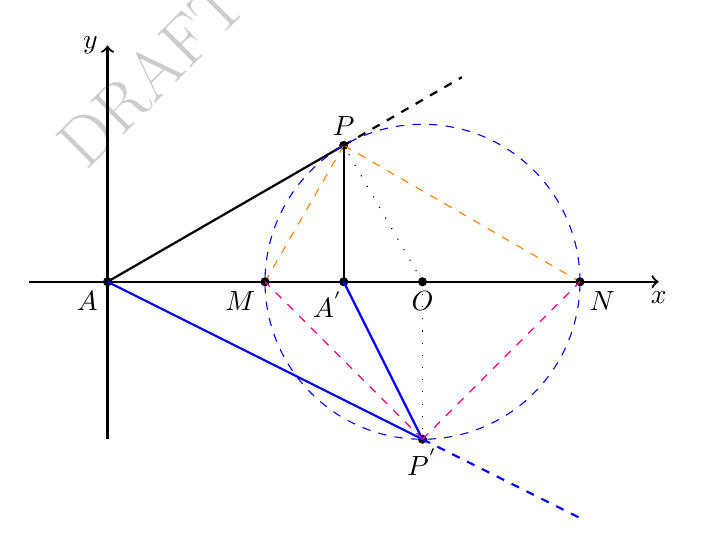
\begin{tikzpicture}
    \draw [fill] (0, 0) circle [radius=0.05];
    \node [below left] at (0, 0) {\(A\)};
    \draw [thick, ->] (0, -2) -- (0, 3);
    \node [left] at (0, 3) {\(y\)};
    \draw [thick, ->] (-1, 0) -- (7, 0);
    \node [below] at (7, 0) {\(x\)};
    \draw [thick] (0, 0) -- (3, 1.732);
    \draw [dashed, thick] (3, 1.732) -- ($(0, 0)!(6, 0)!(3, 1.732)$);
    \node [above] at (3, 1.732) {\(P\)};
    \draw [fill] (3, 1.732) circle [radius=0.05];
    \draw [dashed, blue] (4, 0) circle [radius=2];
    \draw [fill] (4, 0) circle [radius=0.05];
    \node [below] at (4, 0) {\(O\)};
    \draw [dashed, orange](3, 1.732) -- (2, 0);
    \node [below left] at (2, 0) {\(M\)};
    \draw [fill] (2, 0) circle [radius=0.05];
    \draw [dashed, orange](3, 1.732) -- (6, 0);
    \node [below right] at (6, 0) {\(N\)};
    \draw [fill] (6, 0) circle [radius=0.05];
    \draw [fill] (3, 0) circle [radius=0.05];
    \node [below] at (2.8, 0) {\(A^{'}\)};
    \draw [thick] (3, 1.732) -- (3, 0);
    \draw [fill] (4, -2) circle [radius=0.05];
    \node [below] at (4, -2) {\(P^{'}\)};
    \draw [thick, blue] (0, 0) -- (4, -2);
    \draw [dashed, thick, blue] (4, -2) -- ($ 1.5*(4, -2) $);
    \draw [thick, blue] (3, 0) -- (4, -2);
    \draw [dashed, magenta](4, -2) -- (2, 0);
    \draw [dashed, magenta](4, -2) -- (6, 0);

    \draw [loosely dotted] (4, 0) -- (3, 1.732);
    \draw [loosely dotted] (4, 0) -- (4, -2);

\end{tikzpicture}


\end{document}
